\section{Introduction}

\begin{frame}
\frametitle{Introduction}
\framesubtitle{Channels}
\begin{block}{What are channels?}
Channels are types that facilitate the management of concurrency.
\begin{itemize}
\item They help you avoid the use of events + fields to decide who-can-act-when.
\end{itemize}
\end{block}
\end{frame}

\begin{frame}
\frametitle{Introduction}
\framesubtitle{Channel types}
\begin{block}{Primitive channels}
\begin{itemize}
\item Mutex
\item Semaphore
\item FIFO
\end{itemize}
\end{block}
\pause
\begin{block}{Evaluate-update channels (signals)}
\begin{itemize}
\item Generic signals
\item Resolved signals
\end{itemize}
\end{block}
\pause
\begin{block}{These types are based on generic concepts}
Primitive channels are available in many languages. Signals are familiar to HDL users.
\end{block}

\end{frame}

\section{Primitive channels}

\subsection{Mutex}

\begin{frame}[fragile]
\frametitle{Mutex}
\framesubtitle{Definition and usage}
\begin{block}{The type is \texttt{sc\_mutex}}
Stands for {\bfseries mut}ually {\bfseries ex}clusive.
\begin{itemize}
\item A mutex is designed to be "owned" by only one user at the same time
\end{itemize}
It addresses the requirement of exclusive reservation of a resource (like a fuel pump for multiple cars).
\end{block}
\pause
\begin{block}{Normal usage:}
\vspace{-1em}
{\scriptsize 
\begin{verbatim}
sc_mutex NAME; // Declare the mutex variable
NAME.lock(); // Lock it, wait till unlocked if already locked
NAME.unlock(); // Free it
\end{verbatim}
}
\vspace{-1em}
\end{block}
\end{frame}

\begin{frame}[fragile]
\frametitle{Mutex}
\framesubtitle{Blocking vs non-blocking}
\begin{block}{What if we want to do something while waiting?}
The \texttt{lock()} method would block us while we wait.
\end{block}
\pause
\begin{block}{Solution: only {\em try} to lock}
The \texttt{try\_lock()} method returns immediately, and returns an integer value denoting the success of locking.
\begin{itemize}
\item This is necessary in SystemC methods, since they cannot be blocked.
\end{itemize}
\end{block}
\end{frame}

\begin{frame}[fragile]
\frametitle{Mutex}
\framesubtitle{Example: arbitration of a shared bus}
\begin{block}{Bus class and a blocking method}
\vspace{-1em}
{\scriptsize 
\begin{verbatim}
class SharedBus : public sc_module {
    sc_mutex bus_access;
  public: 
    ...
    void write(int addr, int data) {
      bus_access.lock();
      ... // Perform write
      bus_access.unlock();
    }
};
\end{verbatim}
}
\vspace{-1em}
\end{block}

\begin{block}{Non-blocking method usable in a \texttt{SC\_METHOD} process:}
\vspace{-1em}
{\scriptsize 
\begin{verbatim}
    void grab_bus_method() {
      if (bus_access.tryload() == 0) {
        ... // Access bus
        bus_access.unlock();
      }
    }
\end{verbatim}
}
\vspace{-1em}
\end{block}

\end{frame}

\subsection{Semaphore}

\begin{frame}[fragile]
\frametitle{Semaphore}
\framesubtitle{Definition and usage}

\begin{block}{The type is \texttt{sc\_semaphore}}
\begin{itemize}
\item A semaphore is a sort of a set of mutexes
\item The number of semaphores in a semaphore variable is chosen when the variable is declared
\end{itemize}
It addresses the requirement of exclusive reservation of a pool of resources (like a set of fuel pumps for multiple cars)
\end{block}
\pause
\begin{block}{Usage:}
\vspace{-1em}
{\scriptsize 
\begin{verbatim}
sc_semaphore NAME(COUNT); // Declare the semaphore variable
NAME.wait(); // Lock one semaphore, wait if all COUNT used
int success = NAME.trywait(); // Non-blocking version
int num = NAME.get_value(); // Get the number of free semaphores
NAME.post(); // Free one locked semaphore
\end{verbatim}
}
\vspace{-1em}
\end{block}
\end{frame}

\begin{frame}[fragile]
\frametitle{Semaphore}
\framesubtitle{Example: multiport memory}

{\scriptsize 
\begin{verbatim}
class MultiportMemory : public sc_module {
    sc_semaphore read_ports(3);
    sc_semaphore write_ports(2);
  public: 
    void read(int adddr, int& data) {
      read_ports.wait();
      ... // Perform read
      read_ports.post();
    }
    void write(int addr, const int& data) {
      write_ports.wait();
      ... // Perform write
      write_ports.post();
    }
    ...
};
\end{verbatim}
}

\end{frame}

\subsection{FIFO}

\begin{frame}[fragile]
\frametitle{FIFO}
\framesubtitle{Definition and usage}

\begin{block}{The type is \texttt{sc\_fifo<T>}}
The type may be any other type, from a simple boolean to, e.g., a TCP packet.
\begin{itemize}
\item A FIFO is short for First In First Out, i.e., a queue;
\item An \texttt{sc\_fifo} has also a finite depth (size), defaulting to 16.
\end{itemize}
It addresses the requirement of serving requests in order, while allowing requests to accumulate (like a post office).
\end{block}
\pause
\begin{block}{Usage:}
\vspace{-1em}
{\scriptsize 
\begin{verbatim}
sc_fifo<T> NAME(SIZE); // Declare the FIFO variable
NAME.write(VALUE); // Write a value
NAME.read(VALUE); // Read a value
... = NAME.read(); // Function-style read
boolean success = NAME.nb_read(VALUE); // Non-blocking version
int num = NAME.num_free(); // Number of free spaces for write
int num = NAME.num_available(); // Number of data values for read
\end{verbatim}
}
\vspace{-1em}
\end{block}
\end{frame}

\begin{frame}[fragile]
\frametitle{FIFO}
\framesubtitle{Example: Kahn process network}

{\scriptsize 
\begin{verbatim}
SC_MODULE(KahnPN) {
  ...
  sc_fifo<double> a, b, y;
};

KahnPN::KahnPN() : a(24), b(24), y(48) {
  ...
}

void KahnPN::stimulus_thread() {
  for (int i=0; i!= 1024; i++) {
    a.write(double(rand()/1000));
    b.write(double(rand()/1000));
  }
}
void KahnPN::addsub_thread() {
  while(true) {
    y.write(a.read() + b.read());
    y.write(a.read() - b.read());
  }
}
\end{verbatim}
}
\end{frame}

\section{Evaluate-update channels}

\begin{frame}
\frametitle{Evaluate-update channels}
\framesubtitle{What is evaluation-update?}

\begin{block}{It is related to delayed notification}
Delayed notification applies an event after the current evaluation, even if no time has passed.
\begin{itemize}
\item This zero-time evaluate-update loop is called "delta cycle"
\end{itemize}
\end{block}

\begin{figure}
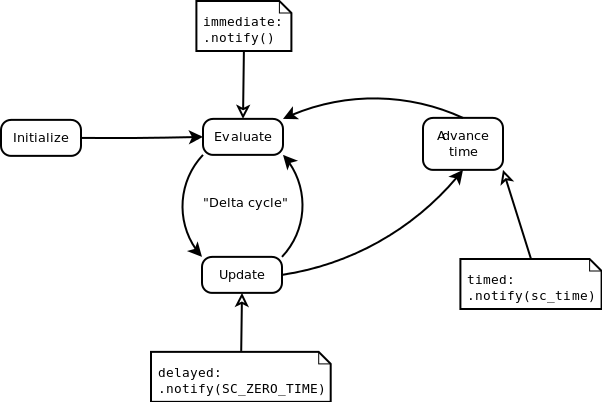
\includegraphics[width=0.65\textwidth]{lecture11/img/simulator.png}
\end{figure}

\end{frame}

\begin{frame}
\frametitle{Evaluate-update channels}
\framesubtitle{Why delayed notification?}

\begin{block}{It allows to trigger value changes}
More specifically, we can design a data type that keeps {\em current} and {next} values.
\end{block}
\pause
\begin{block}{This is necessary when concurrency is considered}
For example, a shift register: each element (i.e., a register) must
\begin{itemize}
\item pass its current value to the next element,
\item get the new value from the previous element
\end{itemize}
where all registers operate concurrently.
\end{block}
\end{frame}

\subsection{Generic signals}

\begin{frame}[fragile]
\frametitle{Generic signals}
\framesubtitle{Definition and usage}

\begin{block}{The type is \texttt{sc\_signal<T>}}
The type \texttt{T} may be any other type.
\begin{itemize}
\item \verb@sc_signal<T> signame;@ \\ Declare a variable
\item \verb@signame.write(VALUE);@ \\ Change the signal value after zero time
\item \verb@signame.read();@ \\ Read the {\em current} value: doesn't immediately reflect a write
\item \verb@wait(signame.value_changed_event());@ \\ Block until the value changes
\item \verb@sensitive << signame;@ \\ Add sensitivity to changes in the signal value
\end{itemize}
Assignment can also be used to read and write, for simplicity.
\end{block}
\end{frame}

\begin{frame}[fragile]
\frametitle{Generic signals}
\framesubtitle{The effect of delta cycles}

{\scriptsize 
\begin{verbatim}
int count;
sc_signal<int> count_sig;
string message;
sc_signal<string message_sig;

count = 11;
cout_sig.write(10);
message = "First";
message_sig.write("Hello");
// The values currently are: 11, 0, "First", ""
wait(SC_ZERO_TIME);
// The values now are: 11, 10, "First", "Hello"
count = 20
count_sig.write(count);
// The values are: 20, 10, "First", "Hello"
wait(SC_ZERO_TIME);
// The values now are: 20, 20, "First", "Hello"
message_sig.write("Hi");
// The values are: 20, 20, "First", "Hello"
wait(SC_ZERO_TIME);
// The values now are: 20, 20, "First", "Hi"
\end{verbatim}
}
\end{frame}

\begin{frame}
\frametitle{Generic signals}
\framesubtitle{Protection from multiple writes}

\begin{block}{Generic signals are not resolved}
Only one process should write on a \texttt{sc\_signal} within one delta cycle. 
The situation where two processes try to write simultaneously ("race condition") is not allowed.
\end{block}
\pause
\begin{block}{This error is not checked by default}
You need to define the \texttt{DEBUG\_SYSTEMC} variable to raise the error on run-time.
\begin{itemize}
\item Remove it again to improve run-time performance, as soon as you verify that your process do not introduce race conditions.
\end{itemize}
\end{block}
\end{frame}

\subsection{Resolved signals}

\begin{frame}[fragile]
\frametitle{Resolved signals}
\framesubtitle{Definition}

\begin{block}{These types operate on \texttt{sc\_logic}:}
\vspace{-1em}
\begin{verbatim}
sc_signal_resolved NAME;  // Scalar
sc_signal_rv<WIDTH> NAME; // Vector
\end{verbatim}
\vspace{-1em}
\end{block}
\pause
\begin{block}{Resolution}
You now can write simultaneously on the same delta cycle, with the following resolution table:

\begin{table}
\begin{tabular}{c|cccc}
\hline
$A\backslash B$ & '0' & '1' & 'X' & 'Z' \\
\hline
'0' & '0' & 'X' & 'X' & '0' \\
'1' & 'X' & '1' & 'X' & '1' \\
'X' & 'X' & 'X' & 'X' & 'X' \\
'Z' & '0' & '1' & 'X' & 'Z'
\end{tabular}
\end{table}
\end{block}
\end{frame}

\begin{frame}[fragile]
\frametitle{Resolved signals}
\framesubtitle{Example of custom resolution: pullup logic}

\begin{block}{We can override the resolution behavior as:}
\vspace{-0.5em}
\begin{table}
\begin{tabular}{c|cccc}
\hline
$A\backslash B$ & '0' & '1' & 'X' & 'Z' \\
\hline
'0' & '0' & 'X' & 'X' & '0' \\
'1' & 'X' & '1' & 'X' & '1' \\
'X' & 'X' & 'X' & 'X' & 'X' \\
'Z' & '0' & '1' & 'X' & {\bfseries '1'}
\end{tabular}
\end{table}
\vspace{-1em}
\end{block}

{\scriptsize 
\begin{verbatim}
struct Pullup : sc_signal_resolved {
  Pullup() : sc_signal_resolved(sc_gen_unique_name("pullup")) {}
  Pullup(const char* nm) : sc_signal_resolved(nm) {}
  
  const sc_logic& read() const {
    const sc_logic& result(sc_signal_resolved::read());
    if (result == SC_LOGIC_Z) 
      return SC_LOGIC_1;
    else
      return result;
  }
};
\end{verbatim}
}
\end{frame}
